\section{Auswertung}
\label{sec:Auswertung}
Für die Ausgleichsrechnung wurden die folgenden Formeln verwendet:

\begin{equation}
	a=\frac{ \overline{xy} - \overline{x} \cdot \overline{y}}{\overline{x^2} - \overline{x}^2}
\end{equation}
\begin{equation}
	b=\frac{\overline{x^2} \cdot \overline{y} - \overline{x} \cdot \overline{xy}}{\overline{x^2} - \overline{x}^2}
\end{equation}
\begin{equation}
	\sigma_y=\sqrt{\frac{1}{N-2}\sum\limits_{i=1}^{N}(y_i - a x_i - b)^2}
\end{equation}
\begin{equation}
	\sigma_a=\sqrt{\frac{\sigma_y^2}{N ( \overline{x^2} - \overline{x} ^2 )}}
\end{equation}
\begin{equation}
	\sigma_b=\sqrt{\frac{\sigma_y^2 \cdot \overline{x}}{N ( \overline{x^2} - \overline{x} ^2 )}}
\end{equation}


	\subsection{Die U/I Graphen der verschiedenen Spannungsquellen}

\subsubsection{Gleichspannungsquelle}
\begin{figure}[H]
	\centering
	\caption{Gleichspannung einer Monozelle}
	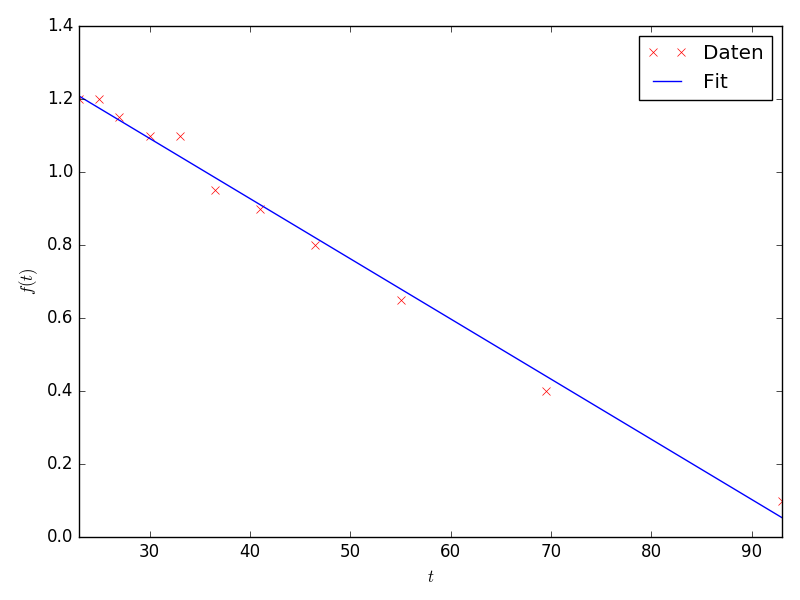
\includegraphics[width=\linewidth-150pt,height=\textheight-150pt,keepaspectratio]{Gleichstrom.png}
	\label{fig:Gleichstrom}
\end{figure}
\begin{table}
	\centering
	\caption{Ergebnisse der Gleichstrommessung ohne Gegenspannung}
	\label{tab:Gleichstrom}
	\sisetup{table-format=1.2}
	\begin{tabular}{S S }
		\toprule
		{$I/$mA} & {$U_k/$V} \\
		\midrule
		23.0 & 1.20 \\
		25.0 & 1.20 \\
		27.0 & 1.15 \\
		30.0 & 1.10 \\
		33.0 & 1.10 \\
		36.5 & 0.95 \\
		41.0 & 0.90 \\
		46.5 & 0.80 \\
		55.0 & 0.65 \\
		69.5 & 0.40 \\
		93.0 & 0.10 \\
		\bottomrule
	\end{tabular}
\end{table}


\subsubsection{ Mit Gegenspannung}

\begin{figure}[H]
	\centering
	\caption{Gleichspannung mit Gegenspannungmethode}
	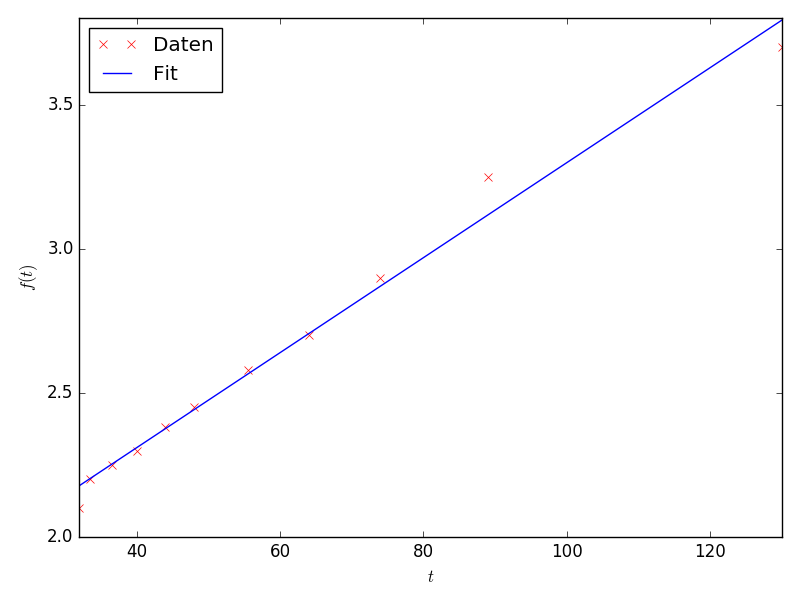
\includegraphics[width=\linewidth-150pt,height=\textheight-150pt,keepaspectratio]{GleichstromR.png}
	\label{fig:GleichstromR}
\end{figure}
\begin{table}
	\centering
	\caption{GleichstromR}
	\label{tab:GleichstromR}
	\sisetup{table-format=1.2}
	\begin{tabular}{S S }
		\toprule
		{$I/mA$} & {$U/V$} \\
		\midrule
		32.0 & 2.1 \\
		33.5 & 2.2 \\
		36.5 & 2.25 \\
		40.0 & 2.3 \\
		44.0 & 2.38 \\
		48.0 & 2.45 \\
		55.5 & 2.58 \\
		64.0 & 2.7 \\
		74.0 & 2.9 \\
		89.0 & 3.25 \\
		130.0 & 3.7 \\
		\bottomrule
	\end{tabular}
\end{table}


\subsubsection{Sinusspannungsquelle}

\begin{figure}[H]
  \centering
  \caption{Der Sinusausgang des RC-Generators}
  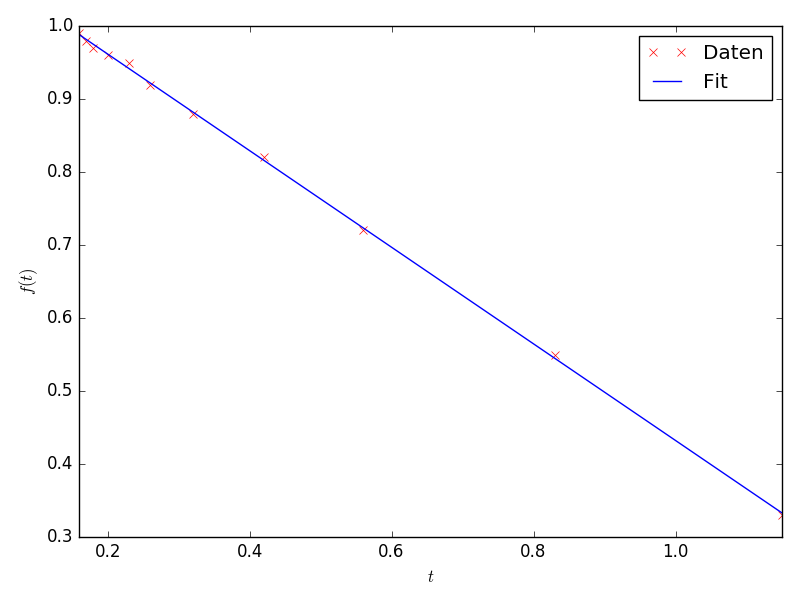
\includegraphics[width=\linewidth-150pt,height=\textheight-150pt,keepaspectratio]{Sinus.png}
  \label{fig:Sinus}
\end{figure}
\begin{table}
	\centering
	\caption{Sinus}
	\label{tab:Sinus}
	\sisetup{table-format=1.2}
	\begin{tabular}{S S }
		\toprule
		{$I/mA$} & {$U/V$} \\
		\midrule
		0.16 & 0.99 \\
		0.17 & 0.98 \\
		0.18 & 0.97 \\
		0.2 & 0.96 \\
		0.23 & 0.95 \\
		0.26 & 0.92 \\
		0.32 & 0.88 \\
		0.42 & 0.82 \\
		0.56 & 0.72 \\
		0.83 & 0.55 \\
		1.15 & 0.33 \\
		\bottomrule
	\end{tabular}
\end{table}

\subsubsection{Rechteckspannungsquelle}

\begin{figure}[H]
	\centering
	\caption{Der Rechteckausgang des RC-Generators }
	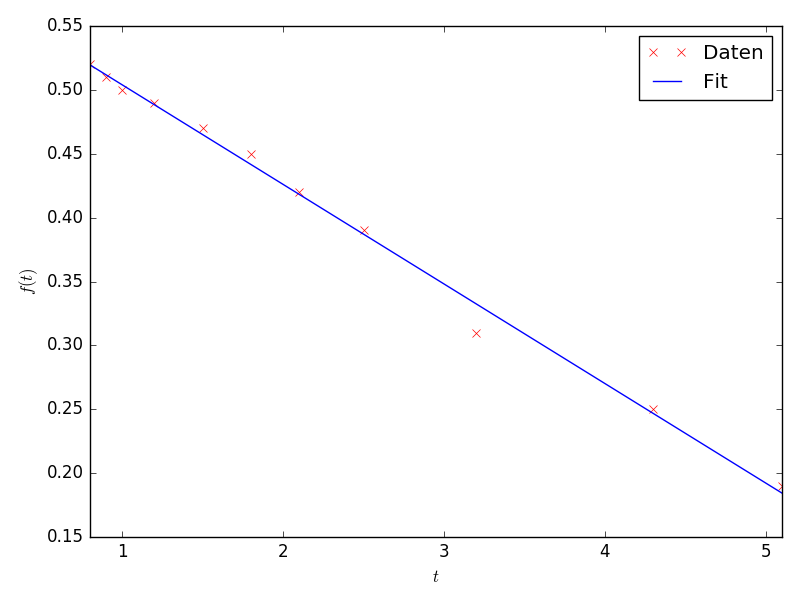
\includegraphics[width=\linewidth-150pt,height=\textheight-150pt,keepaspectratio]{Rechteck.png}
	\label{fig:Rechteck}
\end{figure}
\begin{table}
	\centering
	\caption{Rechteck}
	\label{tab:Rechteck}
	\sisetup{table-format=1.2}
	\begin{tabular}{S S }
		\toprule
		{$I/mA$} & {$U/V$} \\
		\midrule
		0.8 & 0.52 \\
		0.9 & 0.51 \\
		1.0 & 0.5 \\
		1.2 & 0.49 \\
		1.5 & 0.47 \\
		1.8 & 0.45 \\
		2.1 & 0.42 \\
		2.5 & 0.39 \\
		3.2 & 0.31 \\
		4.3 & 0.25 \\
		5.1 & 0.19 \\
		\bottomrule
	\end{tabular}
\end{table}




\begin{figure}[H]
	\centering
	\caption{GleichstromRe.}
	\includegraphics[width=\linewidth-150pt,height=\textheight-150pt,keepaspectratio]{GleichstromRe.png}
	\label{fig:GleichstromRe}
\end{figure}
\cite{scipy}
